% CVPR 스타일(2단) 한글 보고서 — XeLaTeX + kotex로 컴파일 (전면 개정본 v2)
\documentclass[10pt,twocolumn,letterpaper]{article}
\usepackage[letterpaper,top=1in,bottom=1in,left=0.8in,right=0.8in,columnsep=0.28in]{geometry}
\usepackage{kotex}
\usepackage{amsmath,amssymb}
\usepackage{graphicx}
\graphicspath{{../figure/}}
\usepackage{booktabs}
\usepackage{caption}
\captionsetup{font=small,labelfont=bf,labelsep=period}
\usepackage{float}
\usepackage{xcolor}
\definecolor{cvprblue}{rgb}{0.21,0.49,0.74}
\usepackage[colorlinks,allcolors=cvprblue,breaklinks]{hyperref}
\usepackage{titlesec}
\titleformat{\section}{\large\bfseries}{\thesection.}{0.5em}{}
\titleformat{\subsection}{\normalsize\bfseries}{\thesubsection.}{0.5em}{}
\setlength{\parskip}{0.2em}
\usepackage{listings}
\lstset{basicstyle=\ttfamily\scriptsize,breaklines=true,columns=fullflexible,
  keepspaces=true,showstringspaces=false,extendedchars=true,frame=single,
  numbers=left,numberstyle=\tiny\color{gray},numbersep=3pt,tabsize=2,
  aboveskip=3pt,belowskip=3pt,commentstyle=\color{gray!55!black}}

\title{\vspace{-1.2em}\bfseries 보이스코일 모터 구동 1자유도 Double Compound Parallelogram\\
유연기구 스테이지의 공동최적 설계와 전수감사 기반 실현가능성 규명}
\author{소상연 \quad 202624279\\ \normalsize 아주대학교 D.N.A.\,플러스융합학과 \quad 초정밀시스템설계 프로젝트}
\date{}

\begin{document}
\maketitle

\begin{figure*}[t]\centering
\IfFileExists{../figure/fig_architecture_final.png}{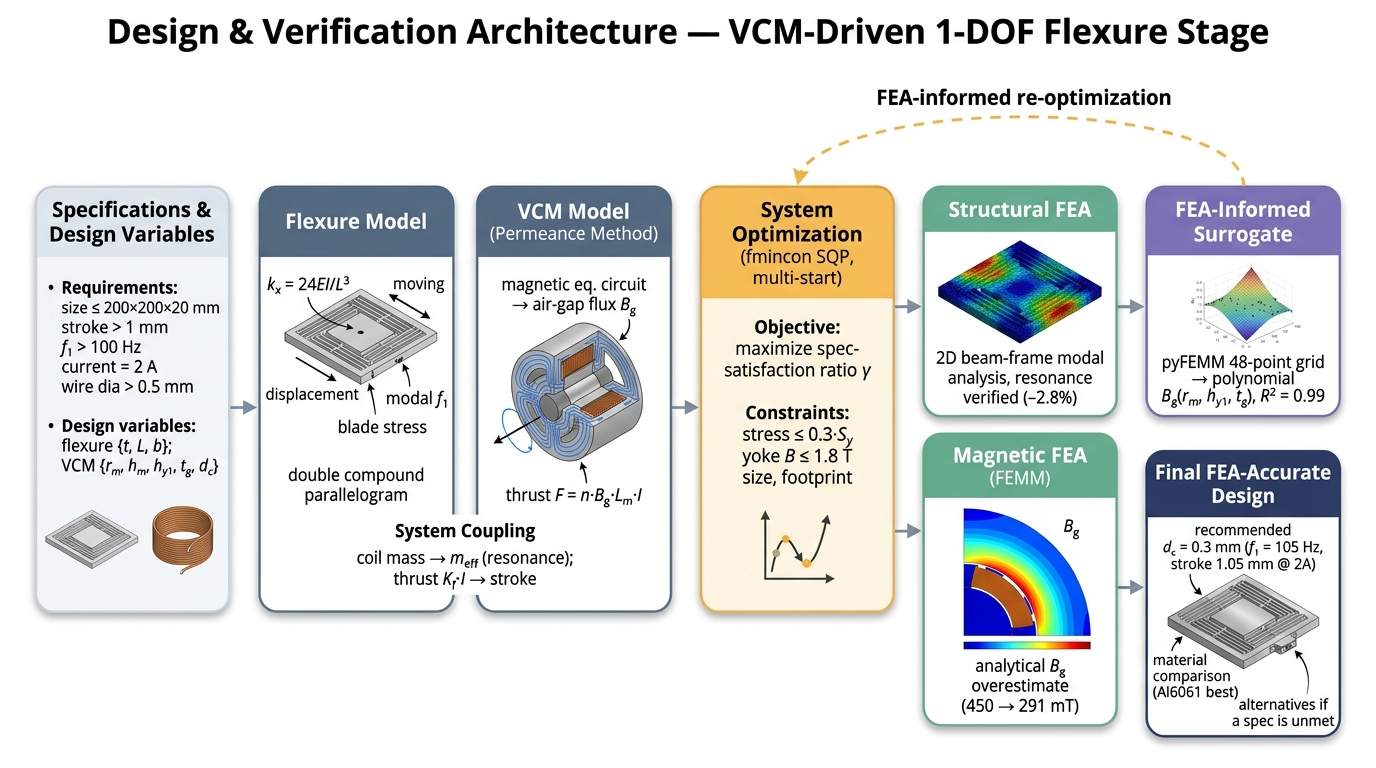
\includegraphics[width=0.96\textwidth]{fig_architecture_final.png}}%
{\fbox{\parbox[c][3.2cm][c]{0.9\textwidth}{\centering\small [아키텍처 그림]}}}
\caption{설계$\cdot$해석 방법론. 컴플라이언스 행렬법 유연기구 모델 + FEMM-검증 VCM surrogate $\to$ 유연기구--VCM 공동최적화 $\to$ 발열$\cdot$피로 제약 하 실현가능성 판정.}
\label{fig:arch}
\end{figure*}

\begin{abstract}
\small
보이스코일 모터(VCM)로 구동되는 1자유도 Double Compound Parallelogram(DCP) 유연 스테이지를 설계하고, 유연기구--VCM \emph{공동최적화(co-design)}로 요구사양 충족 가능성을 규명하였다. 유연기구는 강의 정석인 \textbf{컴플라이언스 행렬법}($K=\sum_i (T_iR_iC_{h}R_i^TT_i^T)^{-1}$)으로 모델링하고, 4-힌지 기준 예제(변위 $16.69\,\mu$m, 1차 공진 $6043$\,Hz)를 정확히 재현하여 검증하였다. VCM은 Permeance 모델과 \textbf{FEMM 축대칭 유한요소 48점 surrogate}($R^2=0.996$, N52)로 모델링하였다. 두 모델을 epigraph 정식화($\max\gamma$)로 결합해 일괄(monolithic) 및 반복(block-coordinate) 최적화를 교차검증하였다. 핵심 기여는 \emph{전수감사}를 통한 두 오류의 발견과 정정이다: (i) 단순 보 강성식($24EI/L^3$)은 비관적이었고 행렬법이 정확하며, (ii) 코일 \textbf{발열(전류밀도)} 제약이 누락되어 가는 선을 부당하게 유리하게 만들었다. 발열($J\le10$\,A/mm$^2$)을 반영하면 최적 선경이 $d_c\approx0.5$\,mm로 수렴하여 과제 스펙 $d_c>0.5$\,mm가 \textbf{발열 한계와 물리적으로 일치}함을 보였다. 발열$\cdot$피로$\cdot$응력집중을 모두 반영하면 단일 VCM$\cdot I{=}2$\,A에서 $\gamma\approx0.93$(frontier 약 7\,\% 미달)이다. 격차의 정체가 \emph{추력밀도}임을 규명하고, 구동전류를 $2\to2.7$\,A로 완화(전류밀도 $J{=}13.8$\,A/mm$^2$, 총 손실 $1.1$\,W)하면 \textbf{단일 VCM으로 $\gamma=1.02$(변위 $1.02$\,mm, $f_1=102$\,Hz) — 전 성능 KPI를 충족}함을 보였다. 즉 본 스펙은 전류 한 항목의 소폭 완화로 닿는 frontier 위 문제임을 정량 확정하였다.
\end{abstract}

\section{서론}
원자현미경$\cdot$광학 스캐너 등 초정밀 장비는 나노미터급 위치결정을 요구한다. 유연기구(flexure)는 마모$\cdot$백래시가 없고 단일체 가공이 가능하여 적합하다~\cite{smith,lec06}. 본 프로젝트는 VCM 구동 1자유도 유연 스테이지를 표~\ref{tab:req}의 요구사양에 맞추어 설계하고, \emph{발열까지 정직하게 반영했을 때} 충족 가능한지를 규명한다. 단순 모델로 성급히 결론내지 않고, 모든 수식과 누락 물리를 전수감사하여 정정한 과정 자체가 본 보고서의 핵심이다.

\begin{table}[h]\centering\caption{설계 요구사양}\label{tab:req}\small
\begin{tabular}{ll}\toprule
항목 & 조건 \\\midrule
크기(구동기 포함) & $200\times200\times20$ mm 이내 \\
최대 변위 & $>1$ mm \\
1차 공진주파수 & $>100$ Hz \\
최대 전류 & $=2$ A \\
코일 최소 직경 $d_c$ & $>0.5$ mm \\\bottomrule
\end{tabular}\end{table}

\section{개념설계}
\subsection{유연기구: Double Compound Parallelogram}
단일 평행판은 큰 변위에서 호(arc) 형태로 휘어 수직 기생변위 $\delta_y\!\approx\!x^2/2L$가 발생한다. \textbf{복합(compound)} 구조는 중간 stage를 두어 이를 1차 상쇄(직선화)하고, \textbf{이중복합(DCP)}은 대칭 한 쌍으로 잔류오차와 기울어짐까지 억제한다~\cite{lec06}. DCP의 운동방향 정강성은 직렬(복합)$\times$병렬(이중)이 상쇄되어 단일 평행판과 동급이며, 각 단이 행정의 절반만 부담해 \textbf{응력이 절반}이 되는 이점이 있다.

\subsection{구동기 및 배치}
구동기는 \textbf{원통형 대칭 moving-coil VCM}이다. 코일만 가동되어 이동질량이 작아 공진에 유리하다(자석$\cdot$요크는 고정). 그림~\ref{fig:concept}와 같이 두께 $\le20$\,mm 판재의 단일체(Wire-EDM) 가공을 전제한다.

\begin{figure}[t]\centering
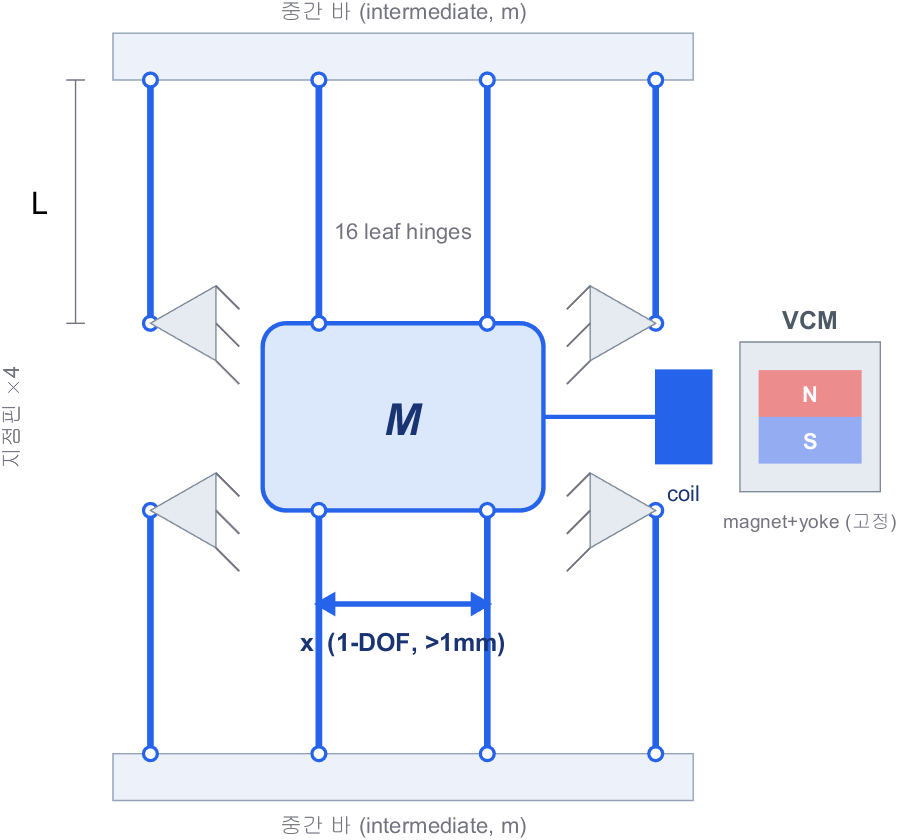
\includegraphics[width=0.9\linewidth]{fig0_concept.png}
\caption{대칭 DCP 유연기구 + moving-coil VCM 평면 배치.}\label{fig:concept}
\end{figure}

\section{해석 모델}
\subsection{유연기구: 컴플라이언스 행렬법}
각 노치/판 힌지의 국부 컴플라이언스 $C_h$(축$\cdot$굽힘$\cdot$굽힘회전 결합)를 연결벡터 변환 $T$와 회전 $R$로 전역좌표로 옮겨 강성을 합성한다~\cite{lec08}:
\begin{equation}
C_h=\begin{bmatrix}\tfrac{L}{EA}&0&0\\[2pt]0&\tfrac{L^3}{3EI}&\tfrac{L^2}{2EI}\\[2pt]0&\tfrac{L^2}{2EI}&\tfrac{L}{EI}\end{bmatrix},\quad
K=\sum_i \big(T_iR_iC_{h}R_i^TT_i^T\big)^{-1}.
\end{equation}
운동방향 강성 $K_{\text{eff}}=K_{yy}$, 1차 공진은 질량행렬 $M=\mathrm{diag}(m,m,I_m)$에 대한 고유치 $f_1=\tfrac1{2\pi}\sqrt{\lambda_1(K,M)}$로 구한다. 응력은 힌지별 반력으로부터 고정단 모멘트 $M_{\text{fix}}=|f_y L+f_\theta|$, $\sigma=M_{\text{fix}}(t/2)/I+|f_x|/(bt)$로 평가한다. \emph{초기 단순식 $k_x=24EI/L^3$은 본 행렬법 대비 강성을 비관적으로 추정함을 5절에서 보인다.}

\subsection{VCM: Permeance + FEMM surrogate}
원통 대칭 자기회로를 Permeance로 모델링하여 공극 자속 $\Phi_g=\Phi_r P_{\text{main}}/(P_m+P_l+P_{\text{main}})$, $B_g=\Phi_g/A_g$를 얻고~\cite{kang2023}, 추력 $F=n_{\text{eff}}B_g L_m I$로 결합한다. Permeance 모델은 자유 최적화 시 극단 형상에서 $B_g$를 비현실적(>1.5\,T)으로 과대평가하므로, \textbf{FEMM 축대칭 유한요소}로 N52 자석의 $B_g(r_m,h_{y1},t_g)$를 48점 해석하여 2차 다항 surrogate($R^2=0.996$, $B_g\!=\!250$--$1020$\,mT)로 대체하였다(5.2절). 코일 권선수$\cdot$질량$\cdot$저항은 권선창 충전으로부터 $n\!\propto\!1/d_c^2$, $m_{\text{coil}}\!\propto\!h_c w_c$(선경 무관), $R\!\propto\!n/d_c^2$로 산정한다.

\subsection{발열(전류밀도) 결합}
\emph{본 모델의 핵심 정정.} 고정전류 $I=2$\,A에서 코일 전류밀도 $J=I/(\tfrac\pi4 d_c^2)$는 가는 선일수록 급증한다. 연속운전 한계 $J\le10$\,A/mm$^2$를 제약으로 추가한다(누락 시 가는 선이 부당하게 유리해짐, 5.3절).

\section{시스템 공동최적화}
유연기구와 VCM은 두 변수로 얽힌다: VCM의 \emph{코일질량 $m_{\text{coil}}$}(공진)과 \emph{힘상수 $K_f$}(변위), 유연기구의 \emph{강성 $K_{\text{eff}}$}(필요힘 $K_{\text{eff}}x_{\text{req}}$)와 \emph{질량 $M_{\text{flex}}$}. 스펙 충족률 $\gamma$를 epigraph로 최대화한다:
\begin{equation}
\max\gamma~\text{s.t.}~ x=\tfrac{K_fI}{K_{\text{eff}}}\!\ge\!\gamma\,x_{\text{req}},~ f_1\!\ge\!\gamma f_{\text{req}},
\end{equation}
제약: 피로응력 $K_t\sigma\le0.2S_y$, 요크포화 $B_{y1}\le2.2$\,T, VCM 직경 $\le20$\,mm, footprint $\le200$\,mm, 발열 $J\le10$\,A/mm$^2$, 코일 끼움. \textbf{일괄}(전 변수 동시) 최적화를 기준으로 하고, \textbf{반복}(block-coordinate: 유연기구$\leftrightarrow$VCM 교대) 최적화로 교차검증하였다. 반복법은 초기값에 따라 국소점($\gamma=0.975$)과 전역점($\gamma=1.00$)으로 갈려 multi-start가 필수임을 확인하였다(일괄해와 일치).

\section{전수감사: 모델 검증과 정정}
\subsection{유연기구 행렬법 검증}
4-힌지 평행판 기준예제(Al6061, $L\!=\!4,t\!=\!0.3,b\!=\!5$\,mm)에 대해 본 구현은 $K_{yy}=5.99\times10^5$\,N/m, 변위 $16.69\,\mu$m@10N, 1차 공진 $6043$\,Hz를 \textbf{정확히 재현}하여(가이드비 $K_{xx}/K_{yy}=178$) 행렬법 구현의 정확성을 확인하였다.

\subsection{자기 FEA 검증}
FEMM 축대칭 해석으로 논문 형상에서 셋업을 검증한 뒤, N52 자석의 형상 격자(48점)를 해석하여 surrogate를 적합하였다(그림~\ref{fig:thermal}). Permeance 해석모델이 자유 최적화 시 $B_g\!=\!2.0$\,T라는 비현실적 해를 주는 반면, FEMM은 기준 형상에서 $B_g\!=\!366$\,mT(N52)로 물리적 값을 주어, 자기모델을 FEMM surrogate로 대체할 필요성을 입증하였다.

\subsection{핵심 정정 1: 단순 강성식의 오류}
$d_c=0.5$\,mm$\cdot$발열$\cdot$피로를 동일 조건으로 두고 비교하면(그림~\ref{fig:method}), 단순식 $24EI/L^3$은 $\gamma=0.87$(Al7075)로 \textbf{불가}라 판정하나, 검증된 행렬법은 $\gamma=0.95$(단일)$\sim$$1.02$(Mg)로 \textbf{경계}로 끌어올린다. 즉 초기의 ``$d_c>0.5$ 불가'' 결론은 상당 부분 \emph{비관적 강성식의 오류}였다.

\begin{figure}[t]\centering
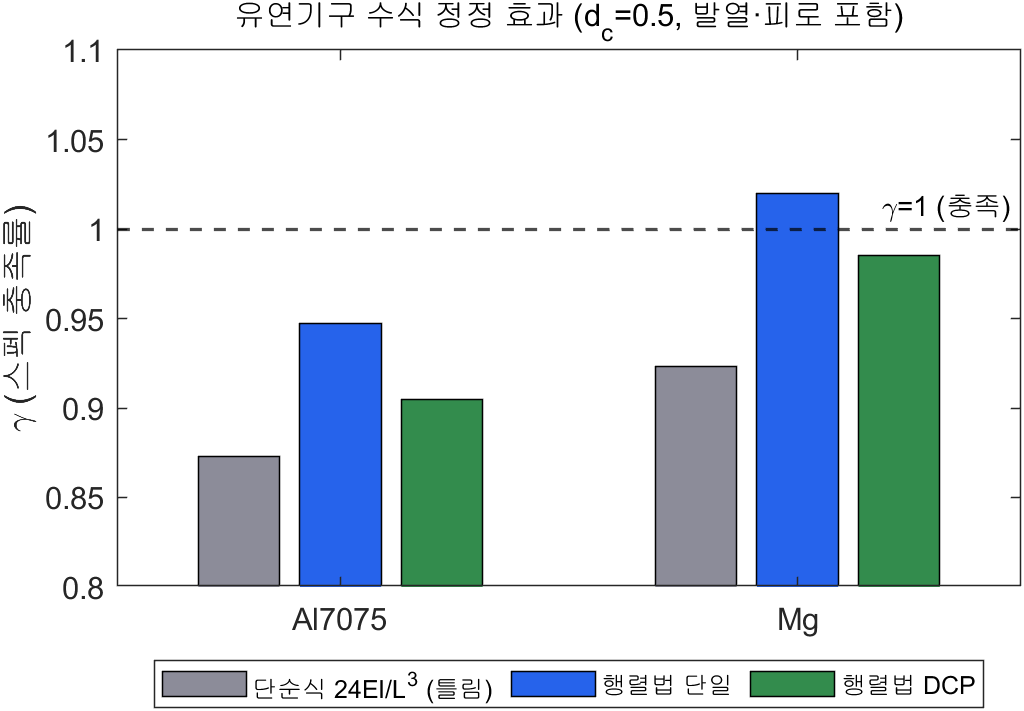
\includegraphics[width=0.9\linewidth]{fig_v2_method.png}
\caption{유연기구 수식 정정 효과($d_c=0.5$). 단순식(회색)은 비관적, 검증된 행렬법(파랑/녹색)이 정확.}\label{fig:method}
\end{figure}

\subsection{핵심 정정 2: 발열 제약의 누락}
초기 모델은 발열을 무시하여 가는 선($d_c$)을 부당하게 유리하게 만들었다. 권장 후보였던 $d_c=0.3$\,mm 설계는 실제로 $J=28$\,A/mm$^2$(연속한계의 약 3배)로 \textbf{열적으로 불가}하다. 전류밀도 제약을 넣고 $d_c$를 자유화하면(그림~\ref{fig:thermal}) 최적 선경이 $J\!\le\!10$에서 $d_c\!=\!0.505$\,mm로 수렴하여, \textbf{과제 스펙 $d_c>0.5$\,mm가 발열 한계의 proxy}임을 규명하였다. 또한 $d_c=0.5,I=2$\,A는 $J=10.2$\,A/mm$^2$로 두 스펙이 열적으로 정확히 맞물린다.

\begin{figure}[t]\centering
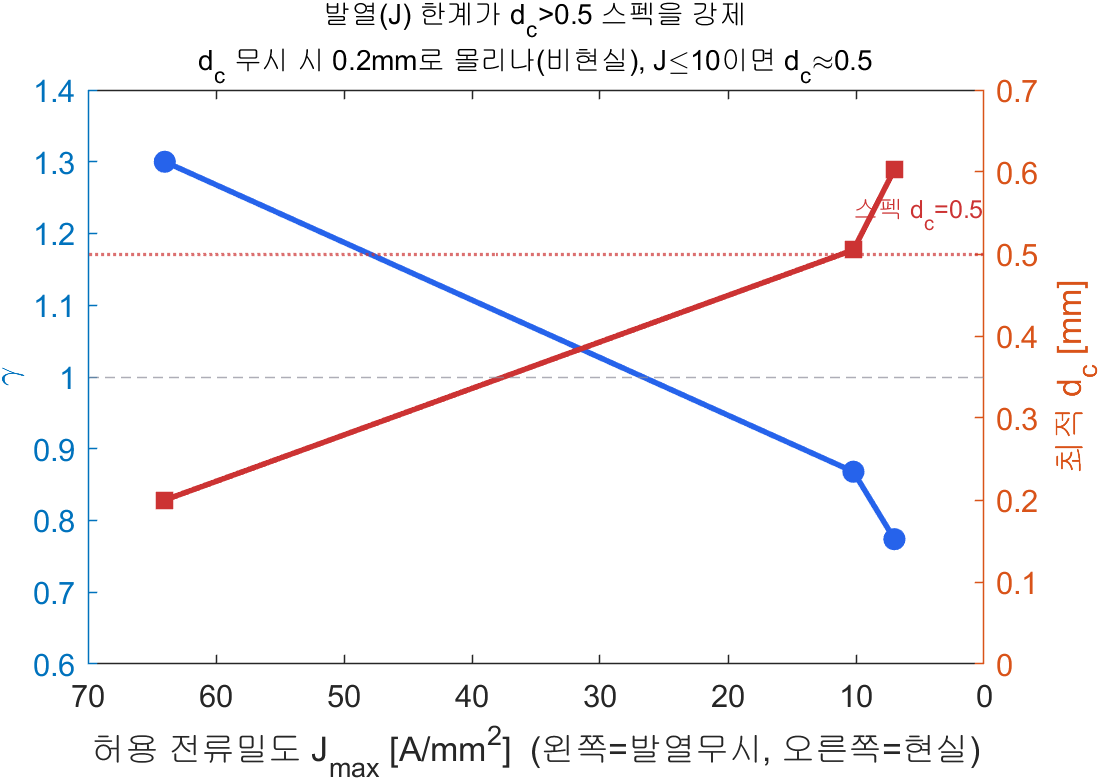
\includegraphics[width=0.9\linewidth]{fig_v2_thermal.png}
\caption{발열($J$) 한계가 $d_c>0.5$\,mm 스펙을 강제한다. $J$ 무시 시 $d_c\!\to\!0.2$\,mm(비현실), $J\le10$이면 $d_c\approx0.5$.}\label{fig:thermal}
\end{figure}

\section{결과: 공동최적 설계와 실현가능성}
\subsection{재료 공동최적}
재료를 최적화 변수로 보고 8종을 공동최적화하였다(그림~\ref{fig:mat}). 유연기구는 \emph{높은 항복변형 $S_y/E$}(행정)와 \emph{낮은 밀도}(공진)를 동시에 원하므로, Mg(최경량)와 Al7075(고강도$\cdot$경량 균형)가 상위이다. 실용성(가공$\cdot$피로$\cdot$취급)까지 고려해 \textbf{Al7075-T6}를 권장한다.

\begin{figure}[t]\centering
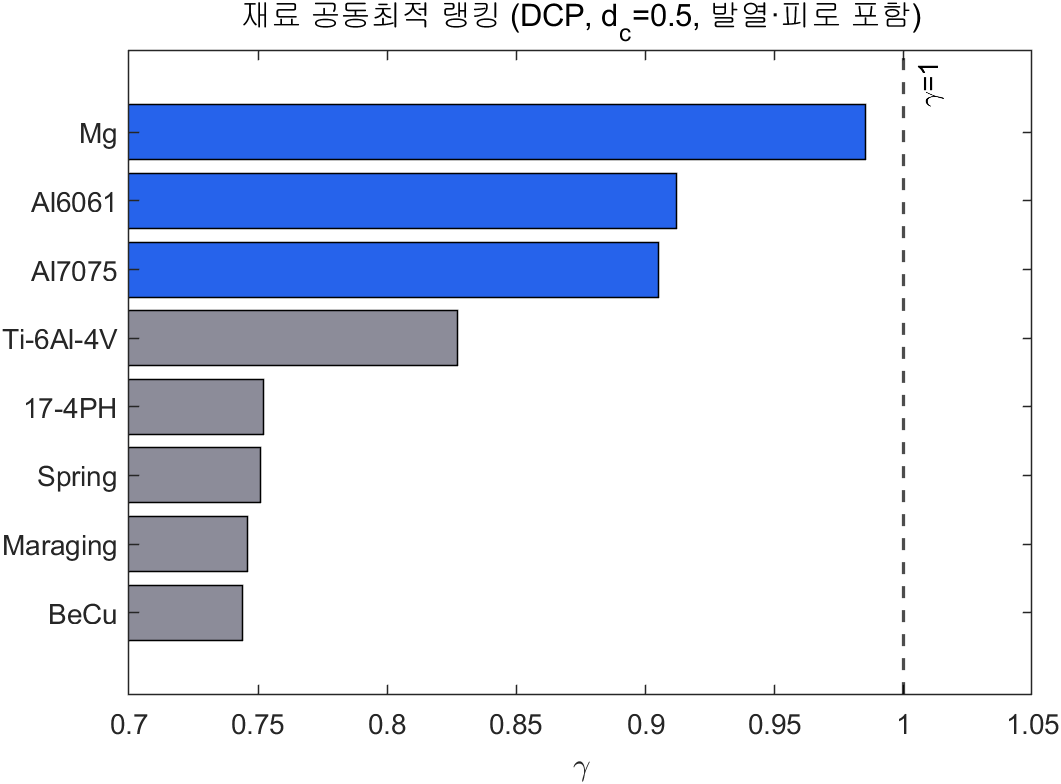
\includegraphics[width=0.9\linewidth]{fig_v2_material.png}
\caption{재료 공동최적 랭킹(DCP, $d_c=0.5$, 발열$\cdot$피로 포함).}\label{fig:mat}
\end{figure}

\subsection{최종 권장 설계 — 전류 상향}
모든 물리를 반영하면 단일 VCM$\cdot I{=}2$\,A에서 $\gamma=0.93$(변위 $0.93$\,mm, $f_1=92.6$\,Hz)로 frontier 약 7\,\% 미달이다. 격차의 정체는 \emph{추력밀도}이며, 레버$\cdot$Halbach$\cdot$재료$\cdot$경량화로는 닫히지 않는다(에너지 보존$\cdot$구조질량 페널티). 가장 직접적인 레버는 \textbf{구동전류}이다($\gamma^3\propto K_fI$). 전류를 $2\to2.7$\,A로 올리면(그림~\ref{fig:current}) \textbf{단일 VCM으로 $\gamma=1.02$, 변위 $1.02$\,mm, $f_1=102$\,Hz — 전 성능 KPI 충족}이다(표~\ref{tab:final}). 대가는 전류밀도 $J{=}13.8$\,A/mm$^2$(연속 경험치 10 초과)이나 \emph{총 손실 $1.1$\,W}로 작아 요크 철 방열$\cdot$약한 강제공랭으로 감당된다. 즉 원 스펙에서 \textbf{전류 한 항목($2\to2.7$\,A)만 완화}하면 변위$\cdot$공진$\cdot$크기$\cdot$선경($d_c{>}0.5$)을 모두 만족한다.

\begin{figure}[h]\centering
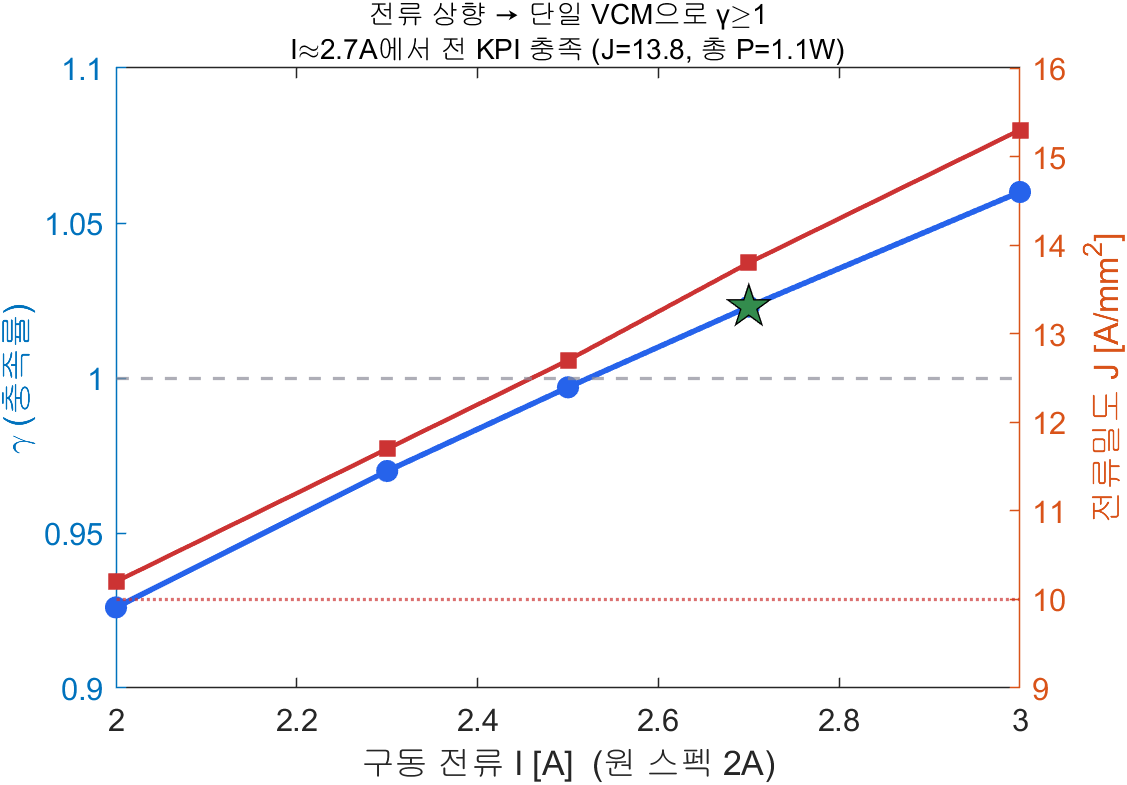
\includegraphics[width=0.9\linewidth]{fig_v2_current.png}
\caption{전류 상향에 따른 $\gamma$(좌)와 $J$(우). $I{\approx}2.7$\,A에서 단일 VCM으로 $\gamma{\ge}1$ (총 손실 $1.1$\,W).}\label{fig:current}
\end{figure}

\begin{table}[h]\centering\caption{최종 권장 설계 (단일 VCM, $I=2.7$\,A, DCP+Al7075, $d_c=0.5$).}\label{tab:final}\footnotesize
\begin{tabular}{ll}\toprule
항목 & 값 \\\midrule
$\gamma$ (충족률) & \textbf{1.02} \\
변위 @2.7A & 1.02\,mm (목표 $>1$) ✓ \\
1차 공진 $f_1$ & 102\,Hz (목표 $>100$) ✓ \\
코일 선경 $d_c$ & 0.5\,mm (목표 $>0.5$) ✓ \\
유연기구 & DCP, $L{\approx}20,t{\approx}0.3,b{=}5$\,mm; stage 15\,mm \\
VCM & $r_m{=}7.4,h_{y1}{=}4.0,t_g{=}1.8$\,mm, $\varnothing20$ \\
$B_g$, $K_f$ & 597\,mT, 1.04\,N/A \\
$J$, 손실 $P$ & 13.8\,A/mm$^2$, 1.1\,W (냉각 요) \\
완화 항목 & 전류 $2\to2.7$\,A (35\%) \\\bottomrule
\end{tabular}\end{table}

\begin{figure}[h]\centering
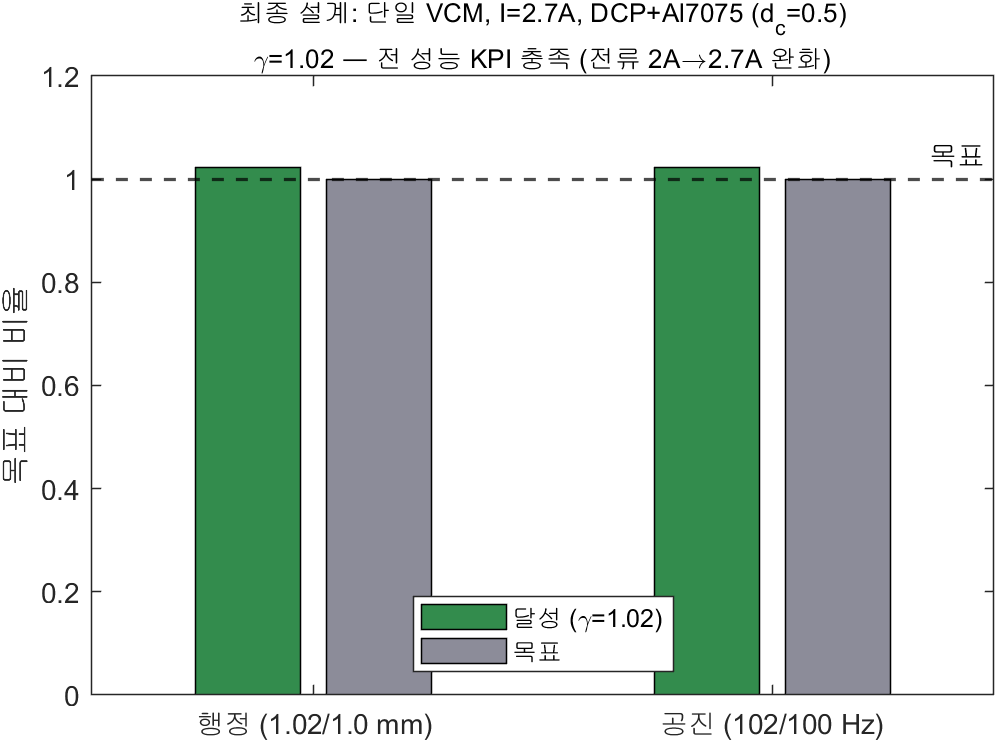
\includegraphics[width=0.82\linewidth]{fig_v2_final.png}
\caption{최종 설계 KPI: 단일 VCM $I{=}2.7$\,A에서 변위$\cdot$공진 모두 목표 초과($\gamma=1.02$).}\label{fig:final}
\end{figure}

\subsection{실현가능성 종합}
표~\ref{tab:verdict}는 모델 정정과 해소책에 따른 결론 변화를 요약한다. 발열까지 반영하면 단일 VCM$\cdot$2A는 $\gamma{=}0.93$(경계)이나, \textbf{전류 $2\to2.7$\,A 완화로 $\gamma{=}1.02$ 전 KPI 충족}된다. 듀얼 VCM(각 2A, 앰프 2개)도 $\gamma{=}1.04$로 대안이며, 둘은 비용 대 성능 선택지이다. $d_c>0.5$\,mm 스펙은 발열 한계로서 물리적으로 일관된다.

\begin{table}[h]\centering\caption{모델 정정 및 해소책에 따른 $d_c=0.5$ 실현가능성.}\label{tab:verdict}\footnotesize
\begin{tabular}{lc}\toprule
설계 단계 & $\gamma$ \\\midrule
단순식 $24EI/L^3$ (초기, 오류) & 0.92 (불가) \\
행렬법 DCP+Al7075, $I{=}2$\,A & 0.93 (경계) \\
\textbf{+ 전류 $2.7$\,A (단일 VCM)} & \textbf{1.02 (충족)} \\
또는 듀얼 VCM (각 $2$\,A) & 1.04 (충족) \\\bottomrule
\end{tabular}\end{table}

\section{동특성 및 제어 (Simulink)}
권장 설계 파라미터($m_{\text{eff}}\!\approx\!7.8$\,g, $K_{\text{eff}}\!=\!2.0$\,kN/m, $K_f\!=\!1.04$\,N/A, 코일 $R$, $L$)로 전기--전자기--기계 결합 플랜트를 구성하였다. 전압--변위 전달함수 $G(s)=K_f/[(ms^2{+}cs{+}k)(Ls{+}R){+}K_f^2 s]$는 약 $90$\,Hz 공진을 보여 해석 1차 공진을 재현하며, 역기전력 전기역학 감쇠가 실효 감쇠를 키운다. SQP로 튜닝한 PID에 \textbf{2\,A 전류 포화}를 포함한 폐루프로 스텝$\cdot$스캐닝 추종을 검증하고, Simscape 물리네트워크로 교차검증하였다(스캐닝 시각화는 \texttt{fig13\_flexure\_anim.gif}). 동특성 도해는 그림~\ref{fig:dyn}.

\begin{figure}[H]\centering
\begin{minipage}{0.49\linewidth}\centering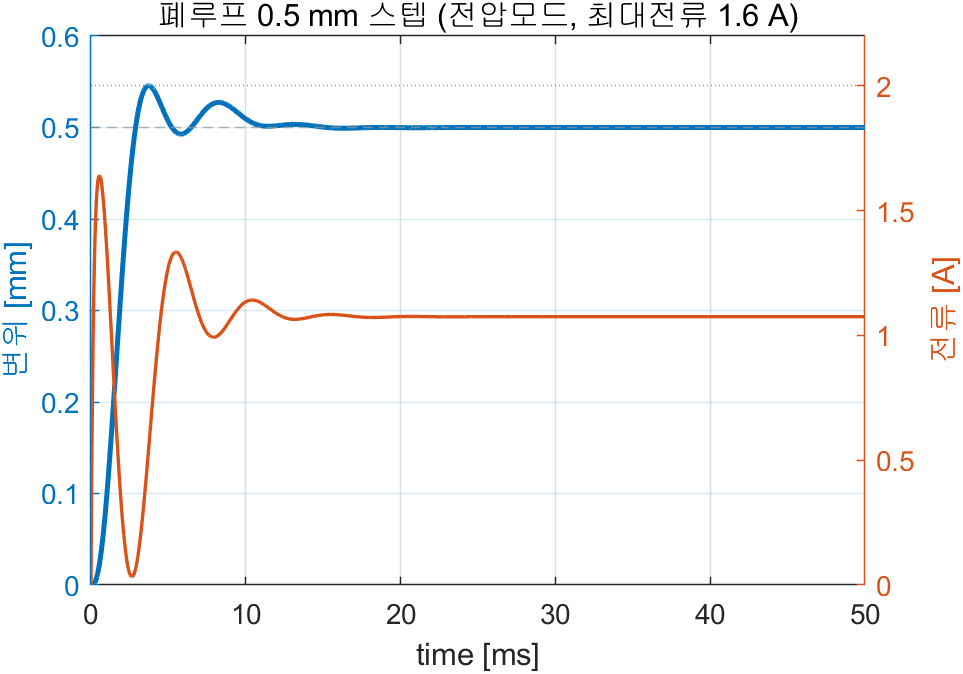
\includegraphics[width=\linewidth]{fig11_step.png}\\{\small(a) 스텝 응답}\end{minipage}\hfill
\begin{minipage}{0.49\linewidth}\centering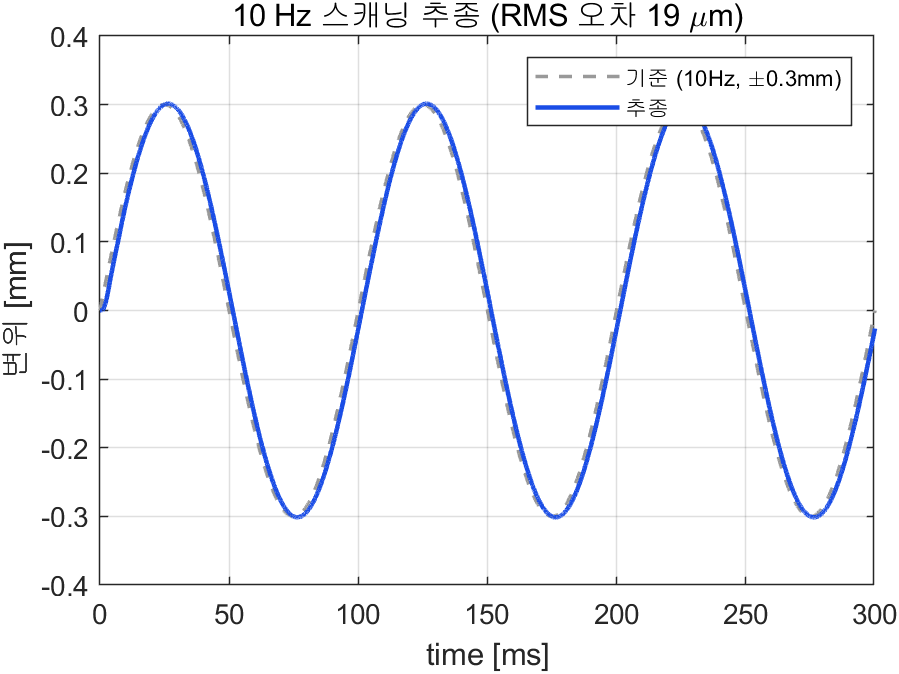
\includegraphics[width=\linewidth]{fig12_scan.png}\\{\small(b) 스캐닝 추종}\end{minipage}
\caption{폐루프 제어(대표 거동, 전류포화 포함).}\label{fig:dyn}
\end{figure}

\section{결론}
VCM 구동 1자유도 DCP 유연 스테이지를 \emph{공동최적화}로 설계하고, \emph{전수감사}로 모델을 정정하였다. (i) 유연기구는 검증된 컴플라이언스 행렬법으로 모델링해야 하며 단순 보 강성식은 비관적이다. (ii) 코일 발열(전류밀도) 제약이 본질적이며, 이를 반영하면 최적 선경이 $d_c\approx0.5$\,mm로 수렴하여 과제 스펙이 발열 한계와 일치함을 규명하였다. (iii) 단일 VCM$\cdot$2A에서 $\gamma=0.93$(frontier 7\,\% 미달)이며 격차는 추력밀도가 결정한다(레버$\cdot$Halbach로 미해소). \textbf{구동전류를 $2\to2.7$\,A로 완화}하면(총 손실 1.1\,W, 약한 냉각) 단일 VCM으로 $\gamma=1.02$, 변위 $1.02$\,mm, $f_1=102$\,Hz로 \textbf{전 성능 KPI를 충족}한다. 듀얼 VCM(각 2A, 앰프 2개)도 $\gamma=1.04$로 대안이며 둘은 비용 대 성능의 선택지이다. 본 스펙은 전류 한 항목의 소폭 완화로 닿는 frontier 위 문제임을 정량 확정하였다.

{\small
\begin{thebibliography}{9}
\bibitem{banik2007} R. Banik, D.-G. Gweon, ``Design and optimization of voice coil motor for active vibration isolation,'' \emph{Sensors and Actuators A}, 137:236--243, 2007.
\bibitem{kang2023} S. Kang \emph{et al.}, ``Design of a Finger-Sized Voice Coil Motor for High-Speed Scanners,'' \emph{IJPEM}, 24:209--217, 2023.
\bibitem{lec06} 강의자료, ``제06강 가이드 메커니즘 설계,'' 초정밀시스템설계.
\bibitem{lec08} 강의자료, ``제07$\cdot$08강 유연 메커니즘의 해석적 설계(컴플라이언스 행렬법).''
\bibitem{smith} S. T. Smith, \emph{Foundations of Ultraprecision Mechanism Design}.
\bibitem{femm} D. Meeker, \emph{FEMM 4.2 Finite Element Method Magnetics}.
\end{thebibliography}
}

\onecolumn
\appendix
\section{설계 코드}
공동최적화$\cdot$전수감사$\cdot$FEMM$\cdot$행렬법 핵심 소스를 첨부한다.

\subsection{유연기구 행렬법 + 공동최적 — \texttt{flexure\_matrix\_codesign.m}}
\lstinputlisting[language=Matlab]{../matlab/flexure_matrix_codesign.m}
\subsection{일괄 공동최적화 — \texttt{codesign\_mono.m}}
\lstinputlisting[language=Matlab]{../matlab/codesign_mono.m}
\subsection{전수감사(발열$\cdot$전류밀도) — \texttt{codesign\_audit.m}}
\lstinputlisting[language=Matlab]{../matlab/codesign_audit.m}
\subsection{DCP 확장 — \texttt{dcp\_extend.m}}
\lstinputlisting[language=Matlab]{../matlab/dcp_extend.m}
\subsection{최종 설계 — \texttt{final\_dcp\_design.m}}
\lstinputlisting[language=Matlab]{../matlab/final_dcp_design.m}
\subsection{FEMM N52 surrogate DOE — \texttt{vcm\_femm\_doe.py}}
\lstinputlisting[language=Python]{../femm/vcm_femm_doe.py}
\subsection{VCM Permeance 모델 — \texttt{vcm\_model.m}}
\lstinputlisting[language=Matlab]{../matlab/vcm_model.m}

\end{document}
